

% Options for packages loaded elsewhere
\PassOptionsToPackage{unicode}{hyperref}
\PassOptionsToPackage{hyphens}{url}
%
\documentclass[
  man]{apa6}
\usepackage{lmodern}
\usepackage{amssymb,amsmath}
\usepackage{ifxetex,ifluatex}
\ifnum 0\ifxetex 1\fi\ifluatex 1\fi=0 % if pdftex
  \usepackage[T1]{fontenc}
  \usepackage[utf8]{inputenc}
  \usepackage{textcomp} % provide euro and other symbols
\else % if luatex or xetex
  \usepackage{unicode-math}
  \defaultfontfeatures{Scale=MatchLowercase}
  \defaultfontfeatures[\rmfamily]{Ligatures=TeX,Scale=1}
\fi
% Use upquote if available, for straight quotes in verbatim environments
\IfFileExists{upquote.sty}{\usepackage{upquote}}{}
\IfFileExists{microtype.sty}{% use microtype if available
  \usepackage[]{microtype}
  \UseMicrotypeSet[protrusion]{basicmath} % disable protrusion for tt fonts
}{}
\makeatletter
\@ifundefined{KOMAClassName}{% if non-KOMA class
  \IfFileExists{parskip.sty}{%
    \usepackage{parskip}
  }{% else
    \setlength{\parindent}{0pt}
    \setlength{\parskip}{6pt plus 2pt minus 1pt}}
}{% if KOMA class
  \KOMAoptions{parskip=half}}
\makeatother
\usepackage{xcolor}
\IfFileExists{xurl.sty}{\usepackage{xurl}}{} % add URL line breaks if available
\IfFileExists{bookmark.sty}{\usepackage{bookmark}}{\usepackage{hyperref}}
\hypersetup{
  pdftitle={Theoretical Bias, as a function of population parameters},
  pdfauthor={Delacre Marie},
  pdfkeywords={keywords},
  hidelinks,
  pdfcreator={LaTeX via pandoc}}
\urlstyle{same} % disable monospaced font for URLs
\usepackage{graphicx,grffile}
\makeatletter
\def\maxwidth{\ifdim\Gin@nat@width>\linewidth\linewidth\else\Gin@nat@width\fi}
\def\maxheight{\ifdim\Gin@nat@height>\textheight\textheight\else\Gin@nat@height\fi}
\makeatother
% Scale images if necessary, so that they will not overflow the page
% margins by default, and it is still possible to overwrite the defaults
% using explicit options in \includegraphics[width, height, ...]{}
\setkeys{Gin}{width=\maxwidth,height=\maxheight,keepaspectratio}
% Set default figure placement to htbp
\makeatletter
\def\fps@figure{htbp}
\makeatother
\setlength{\emergencystretch}{3em} % prevent overfull lines
\providecommand{\tightlist}{%
  \setlength{\itemsep}{0pt}\setlength{\parskip}{0pt}}
\setcounter{secnumdepth}{-\maxdimen} % remove section numbering
\shorttitle{Theoretical Bias}
\affiliation{
\vspace{0.5cm}
\textsuperscript{1} ULB}
\keywords{keywords\newline\indent Word count: X}
\usepackage{csquotes}
\usepackage{upgreek}
\captionsetup{font=singlespacing,justification=justified}

\usepackage{longtable}
\usepackage{lscape}
\usepackage{multirow}
\usepackage{tabularx}
\usepackage[flushleft]{threeparttable}
\usepackage{threeparttablex}

\newenvironment{lltable}{\begin{landscape}\begin{center}\begin{ThreePartTable}}{\end{ThreePartTable}\end{center}\end{landscape}}

\makeatletter
\newcommand\LastLTentrywidth{1em}
\newlength\longtablewidth
\setlength{\longtablewidth}{1in}
\newcommand{\getlongtablewidth}{\begingroup \ifcsname LT@\roman{LT@tables}\endcsname \global\longtablewidth=0pt \renewcommand{\LT@entry}[2]{\global\advance\longtablewidth by ##2\relax\gdef\LastLTentrywidth{##2}}\@nameuse{LT@\roman{LT@tables}} \fi \endgroup}


\DeclareDelayedFloatFlavor{ThreePartTable}{table}
\DeclareDelayedFloatFlavor{lltable}{table}
\DeclareDelayedFloatFlavor*{longtable}{table}
\makeatletter
\renewcommand{\efloat@iwrite}[1]{\immediate\expandafter\protected@write\csname efloat@post#1\endcsname{}}
\makeatother
\usepackage{lineno}

\linenumbers

\title{Theoretical Bias, as a function of population parameters}
\author{Delacre Marie\textsuperscript{1}}
\date{}

\begin{document}
\maketitle

\hypertarget{the-bias}{%
\section{The bias}\label{the-bias}}

For all estimators, when the population effect size is null so is the bias. We will therefore focus on configurations where there is a non-null population effect size. The sampling distribution of Cohen's \(d_s\) (and therefore its bias) is only known under the assumptions of normality and homoscedasticity. On the other side, the biases of Glass's \(d_s\), Cohen's \(d'_s\) and Shieh's \(d_s\) are theoretically known for all configurations where the normality assumption is met, whatever variances are equal across groups or not. In order to simplify the analysis of their bias, it is convenient to subdivise all configurations into 3 conditions:\\
- when variances are equal across populations;\\
- when variances are unequal across populations, with equal sample sizes;\\
- when variances are unequal across populations, with unequal sample sizes.

\hypertarget{preliminary-note}{%
\subsection{Preliminary note}\label{preliminary-note}}

For all previously mentioned estimators (Cohen's \(d_s\), Glass's \(d_s\), Cohen's \(d'_s\) and Shieh's \(d_s\)), the theoretical expectancy is computed by multiplying the population effect size by the following multiplier coefficient:

\begin{equation} 
\gamma=\frac{\sqrt{\frac{df}{2}} \times \Gamma{\frac{df-1}{2}}}{\Gamma{\frac{df}{2}}}
\label{eq:mc}
\end{equation}

Where \(df\) are the degrees of freedom. \(\gamma\) is \emph{always} positive, meaning that when the population effect size is not zero, all estimators will overestimate the real population effect size. Moreover, it is monotonically decreasing and tends to 1 when the degrees of freedom (\(df\)) tend to infinity (\(1.38 \ge \gamma > 1 \; for \; 3 \le df < \infty\); Huynh, 1989). As a consequence, the larger \(df\), the lower the bias.

\hypertarget{cohens-d_s-see-table-1-in-the-article}{%
\subsection{\texorpdfstring{Cohen's \(d_s\) (see Table 1 in the article)}{Cohen's d\_s (see Table 1 in the article)}}\label{cohens-d_s-see-table-1-in-the-article}}

Under the assumptions that independant residuals are normally distributed with equal variances, the \textbf{bias} of Cohen's \(d_s\) is a function of total sample size (N) and the population effect size (\(\delta_{Cohen}\)):

\begin{itemize}
\tightlist
\item
  The larger the population effect size, the more Cohen's \(d_s\) will overestimate \(\delta_{Cohen}\);
\end{itemize}

\begin{figure}
\centering
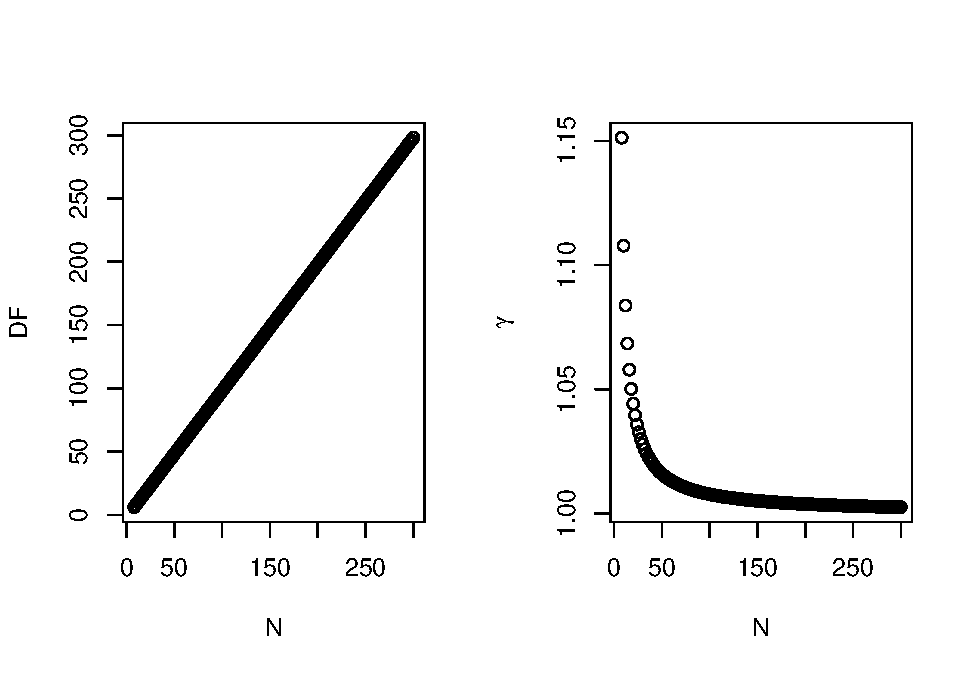
\includegraphics{Theoretical-Bias-of-all-estimators-as-a-function-of-population-parameters_files/figure-latex/biascohendNsize2-1.pdf}
\caption{\label{fig:biascohendNsize2}Degrees of freedom (DF) and \(\gamma\), when computing the bias of Cohen's \(d_s\), when variances are equal across groups, as a function of the total sample size (N)}
\end{figure}

\begin{itemize}
\item
  The larger the total sample size, the lower the bias (see Figure \ref{fig:biascohendNsize2});
\item
  Of course, considering the degrees of freedom, the sample size ratio does not matter (i.e.~the bias will decrease, whatever one increases \(n_1\), \(n_2\) or both sample sizes).
\end{itemize}



\end{document}
